\subsection{Specifications and Requirements}
This project idea requires the integration of power, systems, computer, optical, and web engineering to achieve a final product of a self-sustaining plant bed. The design in \autoref{fig:overall-block} shows four different subsystems the team has designated as power, control, sensing, and web.

\paragraph{Control}
The control subsystem is the brains of the entire operation. This subsystem has to accomplish four distinct tasks:
\begin{enumerate}
    \item Actuate mechanical components (linear rail, solenoid valve)
    \item Convert analog sensor data to digital data
    \item Send plant bed telemetry to web subsystem
    \item Receive commands from web subsystem and modify system accordingly
\end{enumerate}
In order to accomplish the first task, the chosen microcontroller (MCU) must be capable of driving the currents for these components and also support pulse-width modulation (PWM) for interacting with the motor controller. The second task requires that the MCU have an analog-to-digital converter. The third and fourth tasks necessitate WiFi connectivity as well as firmware support for either HTTP requests or WebSockets. These requirements for the control subsystem weigh heavily in the discussion of which MCU to choose found in Section \ref{sec:ps-control}.
\paragraph{Power}
The power system's function is self-explanatory, supply power to the entire system. This will be accomplished in two ways. First, using a DC barrel-plug to the wall, the system could be powered this way. The second way, is via the solar panels, batteries, and charge controller. Both manners of supplying power to the system must be regulated. Discussed Section \ref{sec:ps-power} are the different ways that the charge controller can efficiently switch between battery power and the panels to increase battery health and charge level.
\paragraph{Sensing}

\subsubsection{Engineering Specifications}
\subsubsection{Marketing Requirements}
Find our House of Quality figure below:
\begin{figure}[H]
    \centering
    \caption{House of Quality}
    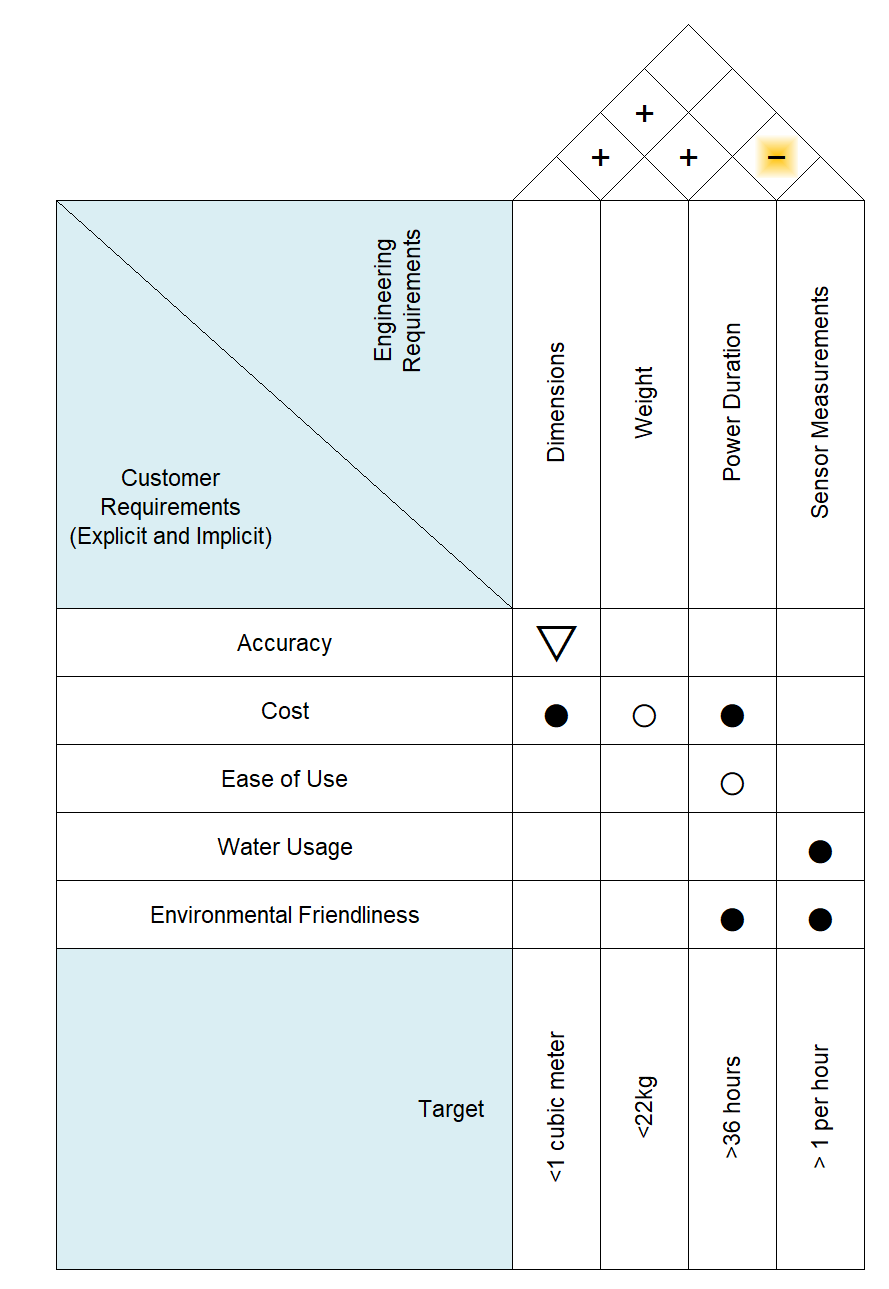
\includegraphics[width=.45\textwidth]{images/HouseOfQuality.PNG}
    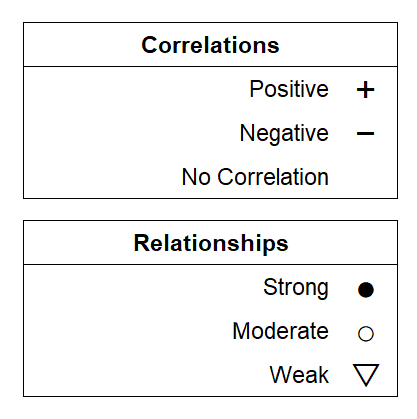
\includegraphics[width=.25\textwidth]{images/HouseOfQualityLegend.png}
\end{figure}
\begin{figure}[H]
    \caption{Overall block diagram}
    \centering
    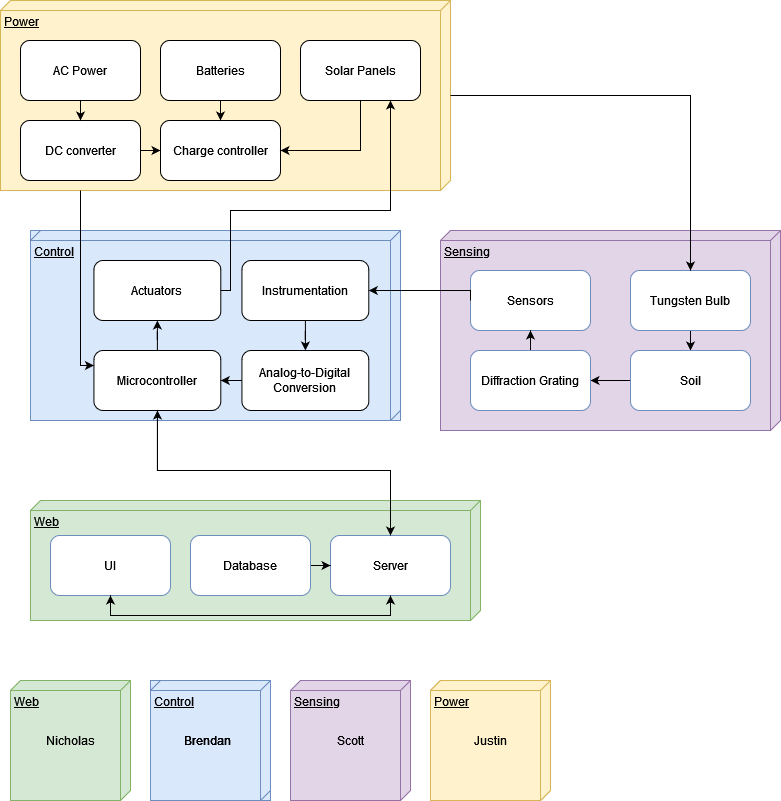
\includegraphics[width=\textwidth]{images/Overall Block Diagram.png}
    \label{fig:overall-block}
\end{figure}